\subsection{\texorpdfstring{$\lambda$}{Лямбда}-исчисление}
\label{sec:lambda}

\paragraph{Историческая справка}
Лямбда-исчисление -- это формальная система, придуманная в 30-ых годах прошлого века Алонзо Черчём~\cite{church1936unsolvable} с целью анализа и формализации понятия вычислимости. В 60-ых годах Питером Ландином была опубликована работа~\cite{landin1964mechanical}, в которой выдвигалась идея о том, что $\lambda$-исчисление может использоваться для моделирования различных выражений в языках программирования того времени, что в дальнейшем привело к развитию языков в стиле \textbf{ML}. С тех пор идеи $\lambda$-исчисления широко используются в мире функционального программирования.

\paragraph{Неформальное описание $\lambda$-термов}
Мы формально определим $\lambda$-термы во второй главе, здесь же мы просто скажем, что термы $\lambda$-исчисления рекурсивно конструируются из переменных с помощью всего двух операций -- применения функции к аргументу и создания анонимной функции. Наличие каких-либо констант здесь не предполагается. Несмотря на кажущуюся простоту, $\lambda$-исчисление является очень мощной формальной системой, в частности, Шейнфинкелем и Карри в работах \cite{schonfinkel1924bausteine, curry1930grundlagen} введен в рассмотрение базис из двух термов(комбинаторов) $S = \lambda f g x. f x (g x)$ и $K = \lambda x y. x$, который примечателен тем, что обладает полнотой по Тьюрингу.

\paragraph{Вариации и расширения}
Изначально, в $\lambda$-исчислении не вводилось никаких правил типизации, однако в дальнейшем появилось множество типизированных вариаций. Барендрегтом в~\cite{barendregt1993lambda} описан так называемый $\lambda$-куб, который наглядно классифицирует восемь различных систем типизации лямбда-исчисления.

\begin{figure}[H]
  \centering
  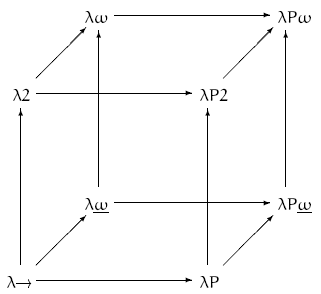
\includegraphics[width=0.5\textwidth]{img/Lambda_cube.png}
  \caption{Лямбда-куб}
\end{figure}

База куба -- просто типизированное $\lambda$-исчисление($\lambda{\to}$), в котором термы могут зависеть только от термов. Три оси соответствуют расширениям, комбинации которых позволяют получить остальные системы типов:

\begin{enumerate}
  \item Термы, которые зависят от типов -- система $\lambda2$ или \textbf{System F}
  \item Типы, которые зависят от типов -- система $\lambda \underline{\omega}$(операторы над типами)
  \item Типы, которые зависят от термов -- система $\lambda P$(зависимые типы)
\end{enumerate}

\paragraph{Соответствие Карри-Говарда}
Затронув системы типизации лямбда-исчисления, нельзя не отметить так называемое соответствие Карри-Говарда~\cite{howard1980formulae}, которое устанавливает прямую связь между логикой и теорией типов. Логической связке соответствует конструкция в теории типов, а логическому утверждению -- тип. Доказательству того факта, что утверждение истинно, соответствует тогда доказательство того факта, что соответствующий этому утверждению тип населен. Иначе говоря, мы можем предъявить $\lambda$-терм соответствующего типа, чтобы доказать исходное утверждение. Для наглядности некоторые соответствия сведены в таблицу:

\begin{table}[H]
  \centering
  \begin{tabular}{| c | c |}
    \hline
    Высказывание $A$: & Тип $A$: \\
    \hline
    Истинно & Населен \\
    \hline
    Тождественная истина & $\top$(единичный тип) \\
    \hline
    Тождественная ложь & $\bot$(пустой тип без обитателей) \\
    \hline
    $\lnot A$(отрицание) & $A \to \bot$ \\
    \hline
    $A \land B$(конъюнкция) & $A \times B$(тип-произведение) \\
    \hline
    $A \lor B$(дизъюнкция) & $A \coprod B$(тип-сумма) \\
    \hline
    $A \to B$(импликация) & $A \to B$(тип функций из $A$ в $B$) \\
    \hline
    $\exists x.P(x)$ & $\Sigma (x : A) (P a)$(тип зависимых пар) \\
    \hline
    $\forall x.P(x)$ & $\Pi (x : A) \to (P a)$(тип зависимых функций) \\
    \hline
  \end{tabular}
  \caption{Соответствия высказываний в логике и конструкций в теории типов}
\end{table}

Чем больше логических связок мы хотим использовать, тем более мощные теории типов  нам придется использовать, чтобы доказывать эти утверждения. Так, например, если нам потребуется доказывать формулы пропозициональной логики, то мы можем обойтись просто типизированным $\lambda$-исчислением. Если нам понадобятся кванторы в формулах, то на помощь приходят теории с зависимыми типами. Благодаря соответствию Карри-Говарда процесс доказательства утверждений становится похож на программирование, следовательно, задача проверки корректности доказательства сводится к задаче проверки типов.

Существует две известные теории с зависимыми типами -- исчисление конструкций(Calculus Of Constructions), представленное Тьерри Коканом в \cite{coquand1988calculus} и интуиционистская теория типов Мартин-Лёфа(Martin-L{\"o}f Type Theory), описанная в \cite{martin1975intuitionistic}. Их расширения лежат в основе таких систем интерактивного доказательства теорем как \textbf{Coq} и \textbf{Agda} соответственно.
